\chapter{التخليق الراجع واستراتيجية الخطوات المتعددة}\label{ch:b2:retrosynthesis}

يُرسم جزيء على السبورة، ولا أحد يعرف بعد كيف يُصنع. وتجريب التفاعلات إلى الأمام، انطلاقًا من
أي شيء على الرف، لا يؤدي إلى شيء: فهي كثيرة جدًا. فيعمل الكيميائي في الاتجاه الآخر، من
الهدف عائدًا نحو الرف، قاطعًا رابطة واحدة في كل مرة على الورق، وكل قطع يلغي تفاعلًا
معروفًا بنجاحه، حتى تصير القطع مركبات يمكن شراؤها. ويحوّل هذا الفصل تفاعلات
الفصول السابقة إلى ذلك الاستدلال الراجع، ثم يسأل كيف يُحكم على الطريق الذي ينتجه.

\begin{recall}
من \cref{ch:b2:alkene-redox} إلى \cref{ch:b2:wittig}: التفاعلات المراد إلغاؤها. ومجلد السنة الأولى:
المجموعات الحامية والأسيتالات، وكواشف غرينيار وانقلاب القطبية، وتخليق ويليامسون،
والانتقائية الكيميائية، وأكسدة الكحولات. والمجلد المدرسي: الاقتصاد الذري.
\end{recall}

\section{التفكير إلى الوراء}

\begin{definition}[التحليل التخليقي الراجع]\label{def:b2:retrosynthesis:analysis}
الجزيء المراد صنعه هو \emph{الجزيء الهدف}\index{جزيء هدف}. و\emph{التحليل التخليقي الراجع}
\index{تحليل تخليقي راجع} يعمل من الهدف عائدًا إلى المواد الأولية المتاحة،
بخطوات كل منها عكس تفاعل معروف؛ وتُكتب الخطوة التخليقية الراجعة بالسهم
المزدوج $\Rightarrow$، ويُقرأ «يُصنع من».
\end{definition}

\begin{definition}[الفك والسنثونات]\label{def:b2:retrosynthesis:disconnection}
\emph{الفك}\index{فك} هو القطع التخيلي لرابطة في الهدف، وهو
عكس تفاعل مكوِّن لرابطة. وقطع رابطة قطعًا غير متجانس يعطي \emph{سنثونين}\index{سنثون}،
وهما شظيتان مشحونتان مثاليتان، إحداهما مانحة (محبة للنواة، سالبة غالبًا)، والأخرى مستقبلة
(محبة للإلكترونات، موجبة غالبًا). و\emph{المكافئ التخليقي}\index{مكافئ تخليقي} كاشف
حقيقي يسلك سلوك سنثون: كاشف غرينيار للأنيون الكربوني \ce{R-}، والألدهيد
للكاتيون $\mathrm{R\overset{+}{C}H{-}OH}$.
\end{definition}

\begin{definition}[تحويل المجموعة الوظيفية]\label{def:b2:retrosynthesis:fgi}
\emph{تحويل المجموعة الوظيفية}\index{تحويل المجموعة الوظيفية} (FGI) خطوة
تخليقية راجعة تغيّر مجموعة وظيفية دون تغيير الهيكل الكربوني: كحول
من كيتون (بالاختزال)، أو سلسلة ألكانية من ألكين (بالهدرجة)، أو أمين من أميد.
\end{definition}

\begin{omfigure}
\begin{tikzpicture}[every node/.style={align=center}]
\node (T) at (0,0) {\setchemfig{atom sep=1.7em}\chemfig{Ph-CH(-[2]OH)-CH(-[6]CH_3)-CH_3}};
\node (A) at (-4.6,-2.6) {\ce{PhCHO}\\[1pt] + \ce{(CH3)2CHMgBr}};
\node (B) at (0,-2.6) {\ce{PhMgBr}\\[1pt] + \ce{(CH3)2CHCHO}};
\node (C) at (4.6,-2.6) {\setchemfig{atom sep=1.7em}\chemfig{Ph-C(=[2]O)-CH(-[6]CH_3)-CH_3}};
\node (D) at (4.6,-5.0) {\ce{C6H6}\\[1pt] + \ce{(CH3)2CHCOCl}};
\draw[omretro] (T.south west) -- node[above left, font=\small] {a} (A.north);
\draw[omretro] (T.south) -- node[right, font=\small] {b} (B.north);
\draw[omretro] (T.south east) -- node[above right, font=\small] {FGI} (C.north);
\draw[omretro] (C.south) -- node[right, font=\small] {c} (D.north);
\end{tikzpicture}
\par\vspace{6pt}

{\small شجرة تخليق راجع للمركب 2-ميثيل-1-فينيل بروبان-1-ول. (a) و(b): الفكّان الممكنان
للرابطة \ce{C-C} المجاورة لكربون الكحول، وكل منهما ألدهيد وكاشف غرينيار. FGI: الكحول
من كيتون، بالاختزال؛ و(c) الكيتون \omterm{def:b2:aromatic-substitution:friedel-crafts}{بأسيلة فريدل--كرافتس} للبنزين. وكل سهم
يُقرأ «يُصنع من».}
\end{omfigure}

تبيّن الشجرة عادات الطريقة. \omterm{def:b2:retrosynthesis:disconnection}{فالفك} يُختار عند رابطة مجاورة لمجموعة وظيفية،
لأن هناك تكوّن التفاعلاتُ الروابطَ. وكل قطع يُفحص بكتابة السنثونات 
وإيجاد كواشف حقيقية لها. ونادرًا ما يكون الجواب واحدًا: فالشجرة تتفرع، والفروع
يُحكم عليها في النهاية (\cref{sec:b2:retrosynthesis:judging}).

\begin{omfigure}
\begin{center}
\small
\renewcommand{\arraystretch}{1.25}
\begin{tabular}{lll}
\hline
\omterm{def:b2:retrosynthesis:disconnection}{السنثون} & النوع & \omterm{def:b2:retrosynthesis:disconnection}{المكافئ التخليقي} \\
\hline
\ce{R-} (ألكيل، أريل) & مانح & \ce{RMgBr}، \ce{RLi}، \ce{R2CuLi} (\omterm{def:b2:conjugate-additions:addition-modes}{إضافة مترافقة}) \\
$\mathrm{^-CH_2COR}$ & مانح & أيون إينولات \ce{CH3COR}، أو 3-أوكسوبيوتانوات الإيثيل \\
$\mathrm{^-C{\equiv}N}$ & مانح & \ce{NaCN} \\
$\mathrm{R\overset{+}{C}H{-}OH}$ & مستقبل & الألدهيد \ce{RCHO} \\
$\mathrm{R\overset{+}{C}{=}O}$ & مستقبل & \omterm{def:b2:acyl-substitution:derivative}{كلوريد الأسيل} \ce{RCOCl}، أو إستر \\
\ce{R+} (أولي) & مستقبل & الهاليد \ce{RBr} (استبدال ثنائي الجزيئية) \\
$\mathrm{^+CH_2CH_2COR}$ & مستقبل & الإينون \ce{CH2=CHCOR} (\omterm{def:b2:conjugate-additions:addition-modes}{إضافة مترافقة}) \\
\hline
\end{tabular}
\end{center}

{\small سنثونات شائعة ومكافئاتها التخليقية. السنثونات المانحة أنيونات كربونية، 
والسنثونات المستقبلة كاتيونات كربونية؛ والكواشف الحقيقية تحمل القطبية نفسها دون الشحنة الكاملة.}
\end{omfigure}

\section{الفك عند مجموعة واحدة}

\omterm{def:b2:retrosynthesis:disconnection}{الفك} عند مجموعة واحدة يقطع رابطة مجاورة لمجموعة وظيفية وحيدة. فمن أجل رابطة \ce{C-O} أو \ce{C-N}
في إيثر أو إستر أو أمين، يمر القطع بين الكربون والذرة غير الكربونية: فتكون الذرة غير الكربونية
المانح، والكربون المستقبل (تخليق ويليامسون، أو \omterm{def:b2:acyl-substitution:esterification}{أسترة}، أو تكوين أميد).
ومن أجل رابطة \ce{C-C}، تحدد المجموعة الوظيفية قطبية السنثونات: فبجوار كربون
كحولي، يكون الكربون الكحولي المستقبل (ألدهيد أو كيتون) والكربون الآخر المانح (مركب
عضوي فلزي)؛ وبجوار كربونيل، يكون الكربون $\alpha$ المانح (أيون إينولات).

ومعظم هذه التفاعلات تحتاج إلى مستوى الأكسدة الصحيح في الموضع الصحيح، فتكون تحويلات FGI بين مستويات
الأكسدة أكثر خطوات الطريق شيوعًا: ألكين، كحول، ألدهيد أو كيتون، حمض. وقد تُرك أحدها
مفتوحًا في مجلد السنة الأولى: إيقاف أكسدة كحول أولي عند الألدهيد.

\begin{proposition}[الأكسدات اللطيفة]\label{prop:b2:retrosynthesis:mild-oxidation}
يتأكسد الكحول الأولي إلى الألدهيد، دون أن يستمر حتى الحمض، بمؤكسد مستعمل في
مذيب عضوي لامائي: كلوروكرومات البيريدينيوم في ثنائي كلوروميثان، أو أكسدة سويرن (ثنائي ميثيل
السلفوكسيد المنشط بكلوريد الأوكساليل، ثم ثلاثي إيثيل أمين، في درجة حرارة منخفضة) أو بيريودينان
ديس--مارتن. أما في الماء، فيؤكسده الكروم(VI) أو البرمنغنات إلى الحمض الكربوكسيلي.
\end{proposition}

\begin{proof}[تعليل]
تنزع هذه المؤكسدات هيدروجين الرابطة \ce{C-H} على الكربون الحامل لمجموعة \ce{OH}. والألدهيد
المتكوّن ليس فيه مثل هذه المجموعة. لكن الألدهيد في الماء في توازن مع هيدراته
\ce{RCH(OH)2}، الذي فيه من جديد \ce{OH} على كربون يحمل هيدروجينًا: فيتأكسد الهيدرات
كما يتأكسد الكحول، إلى الحمض. ودون ماء لا يتكوّن هيدرات، فتتوقف الأكسدة عند
الألدهيد.
\end{proof}

\section{الفك عند مجموعتين}

حين يكون للهدف مجموعتان وظيفيتان، يستعمل أفضل \omterm{def:b2:retrosynthesis:disconnection}{فك} عادة كلتيهما: فتُقطع الرابطة
بحيث توجّه إحدى المجموعتين المانح والأخرى المستقبل. والمسافة بين المجموعتين،
معدودة بالكربونات من كربون وظيفي إلى الآخر مع احتسابهما، تبيّن أي تفاعل يُستعمل.

\begin{proposition}[الأنماط وتفاعلاتها]\label{prop:b2:retrosynthesis:patterns}
ترتبط العلاقات بين مجموعتين بتفاعلات الفصول السابقة على النحو الآتي. فالعلاقات
الفردية (1،3 و1،5) توافق القطبيات الطبيعية لكيمياء الكربونيل؛ أما الزوجية (1،4
و1،6) فلا توافقها، وتحتاج إلى انقلاب القطبية أو إلى شطر حلقة.
\end{proposition}


\begin{proof}[تعليل]
في كيمياء الكربونيل يكون كربون الكربونيل مستقبلًا والكربون $\alpha$ مانحًا، ويضيف الإينون
مستقبلًا عند كربونه $\beta$. \omterm{def:b2:enolates-aldol:enolate}{فأيون الإينولات} (مانح عند $\alpha$) على كربونيل (مستقبل عند كربون
الكربونيل) يصل الكربونين 1 و2 من نمط 1،3: \omterm{def:b2:enolates-aldol:aldol}{الألدول} وكلايزن. \omterm{def:b2:enolates-aldol:enolate}{وأيون الإينولات} على الكربون $\beta$
لإينون يبني نمط 1،5: مايكل، ثم روبنسون. ومن أجل نمط 1،4، يترك القطع
كربونًا $\alpha$ مستقبلًا؛ ولا يقدم أي كاشف كربونيلي عادي تلك القطبية، لكن الكيتون $\alpha$-البرومي
يقدمها، لأن البروميد مجموعة مغادرة عند ذلك الكربون. وثنائي الكربونيل 1،6 هو هكسين حلقي مفتوح
\omterm{def:b2:alkene-redox:cleavage}{بالتحلل الأوزوني} (\cref{prop:b2:alkene-redox:ozonolysis})، والهكسين الحلقي يُصنع \omterm{def:b2:frontier-orbitals:diels-alder}{بتفاعل ديلز--ألدر}
(\cref{def:b2:frontier-orbitals:diels-alder}).
\end{proof}

\begin{omfigure}
\begin{center}
\small
\renewcommand{\arraystretch}{1.25}
\begin{tabular}{lll}
\hline
النمط في الهدف & \omterm{def:b2:retrosynthesis:disconnection}{الفك} & التفاعل \\
\hline
كربونيل $\beta$-هيدروكسيلي (1،3) & الرابطة \babelsublr{$\alpha$--$\beta$} & \omterm{def:b2:enolates-aldol:aldol}{إضافة ألدولية} \\
كربونيل $\alpha,\beta$-غير مشبع & \ce{C=C} & \omterm{def:b2:enolates-aldol:aldol}{تكاثف ألدولي} \\
1،3-ثنائي الكربونيل & \babelsublr{C(O)--C$\alpha$} & \omterm{def:b2:enolates-aldol:claisen}{تكاثف كلايزن} \\
1،5-ثنائي الكربونيل & \babelsublr{C$\alpha$--C$\beta$} في المستقبل & \omterm{def:b2:conjugate-additions:michael}{إضافة مايكل} \\
هكس-2-ين حلقي-1-ون & \ce{C=C} الحلقية، ثم رابطة مايكل & \omterm{def:b2:conjugate-additions:robinson}{الإلحاق الحلقي لروبنسون} \\
هكسين حلقي & رابطتا \ce{C-C} حلقيتان & \omterm{def:b2:frontier-orbitals:diels-alder}{تفاعل ديلز--ألدر} \\
ألكين في موضع محدد & \ce{C=C} & \omterm{def:b2:wittig:wittig}{تفاعل فيتيغ} أو HWE \\
1،4-ثنائي الكربونيل & \ce{C-C} المركزية & أيون إينولات + كيتون $\alpha$-هالوجيني \\
1،6-ثنائي الكربونيل & إعادة وصل الطرفين & \omterm{def:b2:alkene-redox:cleavage}{الانشطار التأكسدي} لهكسين حلقي \\
\hline
\end{tabular}
\end{center}

{\small \omterm{def:b2:retrosynthesis:disconnection}{الفك} عند مجموعتين. الستة الأولى تستعمل القطبية العادية: أيون إينولات (مانح) على
كربونيل أو إينون (مستقبل). ويحتاج نمط 1،4 إلى أن يكون كربون $\alpha$ بالنسبة إلى كربونيل
مستقبلًا، عكس دوره المعتاد، وهو ما يقدمه الكيتون $\alpha$-الهالوجيني.}
\end{omfigure}

\begin{method}[تحليل تخليقي راجع]\label{met:b2:retrosynthesis:retrosynthesis}
\begin{enumerate}
  \item عدّد المجموعات الوظيفية للهدف والعلاقات بينها (1،2؛ 1،3؛ \dots).
  \item فكّر في تحويلات FGI التي تعطي نمطًا له \omterm{def:b2:retrosynthesis:disconnection}{فك} جيد (كحول من كيتون، أو
        سلسلة ألكانية من ألكين).
  \item اختر الروابط الاستراتيجية: بجوار مجموعة وظيفية، أو قرب وسط الجزيء، أو عند
        نقطة تفرع أو حيث تتصل حلقة بسلسلة، بحيث تكون القطع متقاربة الحجم.
  \item اكتب السنثونات، ثم مكافئاتها التخليقية؛ وارفض أي قطع لا كاشف حقيقي له.
  \item تحقق من الانتقائية الكيميائية: أي مجموعة أخرى ستتفاعل مع كل كاشف؟ خطط لحماية
        أو غيّر ترتيب الخطوات.
  \item كرر على كل قطعة حتى تصير كلها متاحة؛ ثم اكتب الطريق إلى الأمام، مع الكواشف 
        والظروف.
\end{enumerate}
\end{method}

\section{المجموعات الحامية في الطريق}

كثيرًا ما يحتاج الطريق إلى كاشف كان سيهاجم مجموعة ثانية في الجزيء. وقد حمى مجلد السنة الأولى
الألدهيدات والكيتونات على هيئة أسيتالات. ويختار الطريق بين عدة مجموعات حامية، تُزال كل منها
بظروفها الخاصة: الأسيتالات (تُزال بالحمض المائي)، وإيثرات السيليل للكحولات (تُزال بأيون
الفلوريد)، وإيثرات البنزيل (تُزال بالتحلل الهيدروجيني على البلاديوم)، وكربامات الأمينات مثل
مجموعة \textit{tert}-بيوتوكسي كربونيل (تُزال بالحمض)، والإسترات (تُزال بالقاعدة).

\begin{definition}[الحماية المتعامدة]\label{def:b2:retrosynthesis:orthogonal}
\emph{المجموعات الحامية المتعامدة}\index{مجموعات حامية متعامدة} مجموعة من المجموعات
الحامية يمكن إزالة كل منها بظروف تترك الأخرى كلها سليمة، بحيث يمكن تحرير الوظائف التي تحجبها
واحدة تلو الأخرى، بأي ترتيب.
\end{definition}

\begin{method}[الحماية في طريق]\label{met:b2:retrosynthesis:protect-in-route}
\begin{enumerate}
  \item لكل خطوة، عدّد المجموعات التي سيهاجمها الكاشف إلى جانب المجموعة المقصودة.
  \item حاول أولًا تجنب الحماية: غيّر ترتيب الخطوات، أو استعمل كاشفًا أكثر \omterm{def:b2:continuous-reactors:selectivity}{انتقائية}
        (بوروهيدريد بدل هيدريد لكيتون بجوار إستر).
  \item وإلا فاختر مجموعة مستقرة في كل خطوة حتى إزالتها، ويمكن إزالتها في ظروف
        يتحملها الجزيء.
  \item مع عدة مجموعات تُحرَّر كل منها على حدة، اختر مجموعة متعامدة.
  \item ابحث عن خطوة تزيل مجموعة مجانًا: فالهدرجة المخطط لها أصلًا تزيل أيضًا
        إيثر البنزيل.
  \item احسب: كل حماية تكلف خطوتين ومردوديهما.
\end{enumerate}
\end{method}

\section{الحكم على طريق}\label{sec:b2:retrosynthesis:judging}

\begin{proposition}[المردود الإجمالي]\label{prop:b2:retrosynthesis:overall-yield}
المردود الإجمالي لسلسلة خطية من الخطوات هو جداء مردودات الخطوات:
$\rho = \rho_1 \rho_2 \cdots \rho_n$. ومع $n$ خطوة متساوية المردود $\rho_1$، $\rho = \rho_1^{\,n}$.
\end{proposition}

\begin{proof}
تحوّل الخطوة $k$ الكمية $n_{k-1}$ من مادتها الأولية إلى $n_k = \rho_k\, n_{k-1}$ من الناتج
(المردودات محسوبة على كميات المركب الوسيط، وكل الكواشف الأخرى بكمية كافية). وبالاستقراء،
$n_n = \rho_n \rho_{n-1} \cdots \rho_1\, n_0$، والمردود الإجمالي $n_n/n_0$ هو الجداء.
\end{proof}

\begin{omfigure}
\begin{tikzpicture}
\begin{axis}[width=0.75\linewidth, height=5.4cm, xmin=0, xmax=20, ymin=0, ymax=100,
  xlabel={\foreignlanguage{arabic}{عدد الخطوات $n$}}, ylabel={\foreignlanguage{arabic}{المردود الإجمالي \babelsublr{(\%)}}}, label style={font=\small},
  tick label style={font=\scriptsize}, xtick={0,5,10,15,20}, grid=major, grid style={black!12},
  legend style={font=\scriptsize, at={(0.98,0.98)}, anchor=north east}, legend cell align=left]
\addplot[omDef, thick] table[x=n, y=r95] {figdata/out/bachelor-2-overall-yield.dat};
\addplot[omThm, thick] table[x=n, y=r90] {figdata/out/bachelor-2-overall-yield.dat};
\addplot[omMeth, thick] table[x=n, y=r80] {figdata/out/bachelor-2-overall-yield.dat};
\addplot[black!60, thick, dashed] table[x=n, y=r70] {figdata/out/bachelor-2-overall-yield.dat};
\legend{\foreignlanguage{arabic}{\babelsublr{95~\%} لكل خطوة}, \foreignlanguage{arabic}{\babelsublr{90~\%} لكل خطوة}, \foreignlanguage{arabic}{\babelsublr{80~\%} لكل خطوة}, \foreignlanguage{arabic}{\babelsublr{70~\%} لكل خطوة}}
\end{axis}
\end{tikzpicture}
\par\vspace{4pt}

{\small المردود الإجمالي لطريق خطي بدلالة عدد خطواته، لأربعة مردودات للخطوة
(\cref{prop:b2:retrosynthesis:overall-yield}). عشر خطوات بمردود 90~\% لكل منها تُبقي 35~\% من المادة؛ 
وعشر خطوات بمردود 70~\%، أقل من 3~\%.}
% figdata: bachelor-2/overall-yield.py
\end{omfigure}

قاعدة الجداء هي سبب فوز الطرق القصيرة، وسبب أن الحماية (خطوتان إضافيتان) ليست مجانية أبدًا، وسبب
تفضيل الكيميائيين بناء نصفين على حدة ووصلهما متأخرين: فيجري الطريق الطويل حينئذ في فرعين
أقصر، ولا تتضاعف خسائر أحد الفرعين بخسائر الآخر. وإلى جانب المردود 
والطول، يُحكم على الطريق \omterm{def:b2:continuous-reactors:selectivity}{بالانتقائية} (يجب أن تعطي كل خطوة ناتجًا واحدًا)، وبكلفة كواشفه وخطورتها،
وبالنفايات التي ينتجها (الاقتصاد الذري لكل خطوة ومذيبات
التنقية)، وبسهولة نقل كل خطوة إلى المقياس الكبير.

\begin{history}[العمل إلى الوراء، بقواعد صريحة]
\begin{minipage}[t]{0.2\linewidth}
\vspace{0pt}
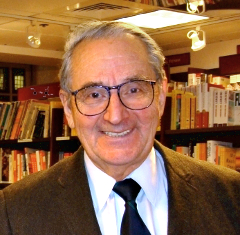
\includegraphics[width=\linewidth]{images/book3/corey.jpg}
\end{minipage}\hfill
\begin{minipage}[t]{0.76\linewidth}
\vspace{0pt}
لطالما استدل الكيميائيون إلى الوراء انطلاقًا من أهدافهم، لكن إلياس جيمس كوري، منذ الستينيات،
حوّل هذه العادة إلى قواعد صريحة: \omterm{def:b2:retrosynthesis:disconnection}{الفك}، \omterm{def:b2:retrosynthesis:disconnection}{والسنثون}، والسهم التخليقي الراجع، 
وحتى برامج حاسوبية تطبقها. ونال جائزة نوبل في الكيمياء لسنة 1990 من أجل نظرية
التخليق العضوي ومنهجيته. (صورة: تروثكيم، CC0، ويكيميديا كومنز.)
\end{minipage}
\end{history}

\begin{safety}{\ghs[5mm]{GHS02}\,\ghs[5mm]{GHS03}\,\ghs[5mm]{GHS05}\,\ghs[5mm]{GHS06}\,\ghs[5mm]{GHS07}\,\ghs[5mm]{GHS08}}
كلوريد الأوكساليل أكّال وسام ويتفاعل مع الماء، مطلقًا كلوريد الهيدروجين؛ وأكسدة سويرن
تطلق أحادي أكسيد الكربون وكبريتيد ثنائي الميثيل الكريه الرائحة، فتُجرى تحت ساحبة أبخرة.
وبيريودينان ديس--مارتن مؤكسد ويجب ألا يُسخَّن. وكواشف الكروم(VI) تُتجنب اليوم
حيثما وُجد بديل.
% ledger: ghs:oxalyl-chloride, ghs:DMSO, ghs:DMP
\end{safety}

\section{تمارين}

\begin{exercise}[$\star$]\label{exo:b2:retrosynthesis:1}
فكّك كل كحول إلى مركب كربونيلي وكاشف غرينيار (أعطِ كل الإمكانات):
2-فينيل بروبان-2-ول، البنتان-3-ول، 1-هكسيل حلقي إيثانول، 2-ميثيل بيوتان-2-ول، 1-فينيل إيثانول.
\end{exercise}

\begin{exercise}[$\star$]\label{exo:b2:retrosynthesis:2}
في \omterm{def:b2:retrosynthesis:disconnection}{فك} 1-فينيل إيثانول عند الرابطة \ce{C-C}، سمِّ \omterm{def:b2:retrosynthesis:disconnection}{السنثونين}، وقل أيهما
المانح، وأعطِ مكافئًا تخليقيًا لكل منهما.
\end{exercise}

\begin{exercise}[$\star$]\label{exo:b2:retrosynthesis:3}
لطريق من خمس خطوات مردودات خطوات 90 و85 و80 و95 و70~\%. احسب مردوده الإجمالي.
\end{exercise}

\begin{exercise}[$\star$]\label{exo:b2:retrosynthesis:4}
يجب تحويل 4-أوكسوبنتانوات الإيثيل إلى 5-هيدروكسي بنتان-2-ون. خطط للطريق مع مجموعة
حامية، وقل لماذا تلزم.
\end{exercise}

\begin{exercise}[$\star\star$]\label{exo:b2:retrosynthesis:5}
اقترح تخليقًا راجعًا للبيوتان-1،3-ديول من مركبات فيها ذرتا كربون على الأكثر، مع FGI 
\omterm{def:b2:retrosynthesis:disconnection}{وفك} عند مجموعتين.
\end{exercise}

\begin{exercise}[$\star\star$]\label{exo:b2:retrosynthesis:6}
فكّك 1-(هكس-3-ين حلقي-1-يل)إيثان-1-ون \omterm{def:b2:frontier-orbitals:diels-alder}{بتفاعل ديلز--ألدر}.
\end{exercise}

\begin{exercise}[$\star\star$]\label{exo:b2:retrosynthesis:7}
فكّك 4،4-ثنائي ميثيل هكس-2-ين حلقي-1-ون \omterm{def:b2:conjugate-additions:robinson}{بالإلحاق الحلقي لروبنسون}.
\end{exercise}

\begin{exercise}[$\star\star$]\label{exo:b2:retrosynthesis:8}
يمكن تحضير 1-فينيل بيوتان-1-ون في خطوة واحدة \omterm{def:b2:aromatic-substitution:friedel-crafts}{بأسيلة فريدل--كرافتس}، أو في خطوتين انطلاقًا من البنزالدهيد.
اكتب الطريقين وقارن بينهما.
\end{exercise}

\begin{exercise}[$\star\star$]\label{exo:b2:retrosynthesis:9}
المطلوب الهكسانال انطلاقًا من الهكسان-1-ول. أي الكواشف تعطيه، وأيها كان سيعطي حمض الهكسانويك
بدلًا منه؟ فسّر.
\end{exercise}

\begin{exercise}[$\star\star\star$]\label{exo:b2:retrosynthesis:10}
في 4-أمينوبيوتان-1-ول، يجب أن يتفاعل الأمين أولًا مع \omterm{def:b2:acyl-substitution:derivative}{كلوريد أسيل} في خطوة، والكحول
لاحقًا مع آخر. اقترح زوجًا متعامدًا من المجموعات الحامية والتسلسل.
\end{exercise}

\begin{exercise}[$\star\star\star$]\label{exo:b2:retrosynthesis:11}
اقترح تخليقًا للهكسان-2،5-ديون، وهو مركب 1،4-ثنائي الكربونيل، انطلاقًا من 3-أوكسوبيوتانوات الإيثيل.
\end{exercise}

\begin{exercise}[$\star\star\star$]\label{exo:b2:retrosynthesis:12}
6-ميثيل هبت-5-ين-2-ون، \ce{(CH3)2C=CHCH2CH2COCH3}، مركب وسيط في صناعة العطور. اقترح خطة كاملة
انطلاقًا من 3-أوكسوبيوتانوات الإيثيل وهاليد: التخليق الراجع، والطريق إلى الأمام، والخطوة التي تزيل
الإستر.
\end{exercise}

\section{مسألة: كيتون التوت}

\begin{problem}[{مسألة نهاية الأسبوع --- التخليق الراجع لمركب منكِّه، والفينول وهل
يُحمى، وبديل بالبلاديوم، والحكم على الطرق}]
\label{pb:b2:retrosynthesis:1}
كيتون التوت، 4-(4-هيدروكسي فينيل)بيوتان-2-ون، يوجد في التوت وفواكه أخرى ويُستعمل
منكِّهًا وفي صناعة العطور. معطيات التمرين: مردودات خطوتي الطريق الألدولي، 85~\% (التكاثف)
و92~\% (الهدرجة). والكتل المولية (\unit{g/mol}): C 12.011، H 1.008، O 15.999، N 14.007،
I 126.90. وقيمة $\mathrm pK_a$ للفينول 9.99.
% ledger: use:raspberry-ketone, aw:C, aw:H, aw:O, aw:N, aw:I, pka:phenol, ghs:raspberry-ketone, ghs:4-iodophenol, ghs:MVK

\medskip
\noindent\textbf{الجزء الأول --- التخليق الراجع.}
\begin{enumerate}
  \item ارسم الهدف وسمِّ مجموعاته الوظيفية.
  \item أي FGI يحوّل الوحدة \ce{ArCH2CH2CO} إلى نمط له \omterm{def:b2:retrosynthesis:disconnection}{فك} معروف؟
  \item اكتب الكيتون غير المشبع الناتج، مع هندسته.
  \item أي نمط ثنائي المجموعة يحوي، وأي تفاعل يصنعه؟
  \item سمِّ المادتين الأوليتين.
  \item لماذا يعطي هذا التفاعل الألدولي المتصالب ناتجًا رئيسيًا واحدًا؟
  \item اكتب الطريق إلى الأمام في خطوتين، مع الظروف.
\end{enumerate}

\medskip
\noindent\textbf{الجزء الثاني --- الفينول.}
\begin{enumerate}[resume]
  \item في هيدروكسيد الصوديوم المائي، بأي صورة يوجد 4-هيدروكسي بنزالدهيد؟ استعمل
        قيمة $\mathrm pK_a$.
  \item كيف تغيّر تلك الصورة المحبة للإلكترونات لدى الألدهيد؟
  \item لو حُمي الفينول، فأي مجموعة كانت الخطوة الثانية ستزيلها مجانًا؟ فسّر.
  \item عُدّ خطوات الطريق مع تلك الحماية.
  \item هل تتعرض الحلقة البنزينية للخطر في الهدرجة؟
  \item أنحمي أم لا؟ استنتج.
\end{enumerate}

\medskip
\noindent\textbf{الجزء الثالث --- بديل بالبلاديوم.}
\begin{enumerate}[resume]
  \item فكّك الكيتون غير المشبع عند الرابطة بين الحلقة والسلسلة: أي شريكين في تفاعل
        هيك؟
  \item اكتب تفاعل هيك مع ثلاثي إيثيل أمين قاعدةً.
  \item عند أي كربون من البوت-3-ين-2-ون تنتهي مجموعة الأريل، ولماذا؟
  \item سمِّ خطوات \omterm{def:b2:catalytic-cycles:cycle}{الدورة الحفزية}.
  \item احسب الاقتصاد الذري لخطوة هيك، مع احتساب ثلاثي إيثيل أمين.
  \item احسب الاقتصاد الذري \omterm{def:b2:enolates-aldol:aldol}{للتكاثف الألدولي}.
\end{enumerate}

\medskip
\noindent\textbf{الجزء الرابع --- الحكم على الطرق.}
\begin{enumerate}[resume]
  \item ما الاقتصاد الذري للهدرجة؟
  \item احسب الاقتصاد الذري الإجمالي للطريق الألدولي.
  \item أي رابطة مزدوجة تختزلها الهدرجة، ولماذا يبقى الكيتون؟
  \item قارن كواشف الطريقين من حيث الكلفة والخطورة.
  \item أي طريق تختار؟
  \item ماذا تفعل خطوة ثالثة بمردود 90~\% بالمردود الإجمالي؟
  \item اذكر المردود الإجمالي للطريق الألدولي ذي الخطوتين.
\end{enumerate}
\end{problem}
